\section{Árvores}

\begin{frame}[fragile]{Características das árvores}

    \begin{itemize}
        \item As {árvores} são estruturas compostas de {nós} e {ramos} (arestas)

        \item Ao contrário das árvores reais, a visualização de árvores em algoritmos é 
            {invertida}, com a {raiz} no topo e as {folhas} na base
        
        \item A {raiz} é um nó que {não tem} pai
        
        \item {Folhas} são nós {que não} tem filhos

        \item Cada nó pode ser alcançado atráves de uma sequência {única}
            de ramos, denominada {caminho}
        

        \item O {nível} de um nó $N$ corresponde ao número de nós do caminho de $N$ até a  raiz 

        \item A {altura} de uma árvore é igual ao {nível máximo} dentre todos os nós da árvore

        \item Uma árvore {vazia} tem altura 0 (zero); uma árvore com {um único} nó tem altura 1

    \end{itemize}

\end{frame}  

\begin{frame}[fragile]{Visualização de uma árvore}

    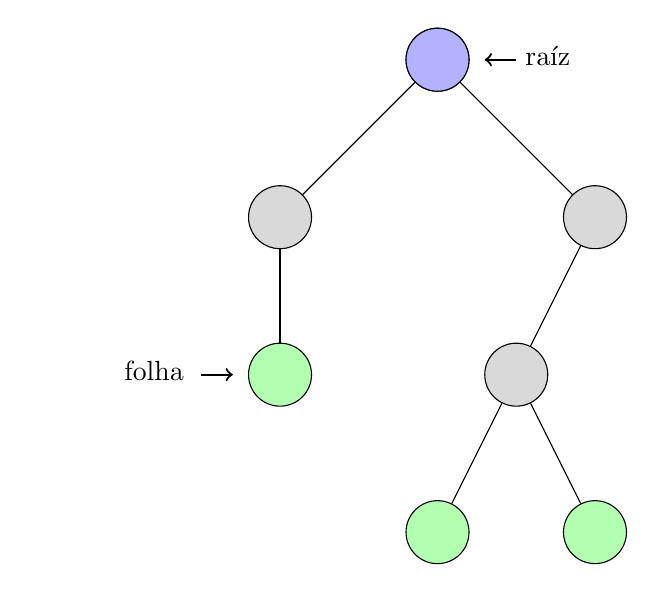
\begin{tikzpicture}
        \begin{scope}{shift={(3,0)}}
            \node[opacity=0] (X) at (-1, 2) { $1$ };
            \node[minimum size=0.8cm, fill=blue!30,circle,draw] (A) at (4, 8) { };
            \node[minimum size=0.8cm, fill=blue!30,circle,draw] (A) at (4, 8) { };
            \node[minimum size=0.8cm, fill=gray!30,circle,draw] (B) at (2, 6) { };
            \node[minimum size=0.8cm, fill=gray!30,circle,draw] (C) at (6, 6) { };
            \node[minimum size=0.8cm, fill=green!30,circle,draw] (D) at (2, 4) { };
            \node[minimum size=0.8cm, fill=gray!30,circle,draw] (E) at (5, 4) { };
            \node[minimum size=0.8cm, fill=green!30,circle,draw] (F) at (4, 2) { };
            \node[minimum size=0.8cm, fill=green!30,circle,draw] (G) at (6, 2) { };

            \draw (A) -- (B);
            \draw (A) -- (C);
            \draw (B) -- (D);
            \draw (C) -- (E);
            \draw (E) -- (F);
            \draw (E) -- (G);

            \draw[thick,->] (5.0, 8) -- (4.6, 8);
            \node at (5.4, 8.05) { raíz };

            \draw[thick,->] (1.0, 4) -- (1.4, 4);
            \node at (0.4, 4.05) { folha };
        \end{scope}
    \end{tikzpicture}

\end{frame}

\begin{frame}

    \frametitle{Definição formal das árvores}

    As {árvores} são estruturas que podem ser definidas recursivamente da seguinte maneira:
    
    \begin{enumerate}
        \item Uma estrutura {vazia} é uma árvore
        

        \item Se $t_1, t_2, \ldots, t_k$ são árvores disjuntas, então a 
        estrutura cuja {raiz} tem como {filhos} as raizes de 
        $t_1, t_2, \ldots, t_k$ também é uma árvore
        

        \item Apenas estruturas {geradas pelas regras} 1 e 2 são 
        árvores
    \end{enumerate}

\end{frame}
